
\newcommand {\matr}[2]{\left[\begin{array}{#1}#2\end{array}\right]}
\newcommand{\E}{\mathbb{E}}
\newcommand{\tr}{\mathrm{tr}}
\newcommand{\x}{{\mathbf{x}}}
\renewcommand{\u}{{\mathbf{u}}}
\newcommand{\w}{{\mathbf{w}}}
\renewcommand{\r}{{\mathbf{r}}}

%%%%%%%%%%%%%%%%%%%%%%%%%%%%%%%%%%%%%%%%%%%%%%%%%%%%%%%%%%%%%%%%%%%%%%%%%%%%%%%%
\begin{abstract}
This paper concerns automated vehicles negotiating with other vehicles, typically human driven, in crossings with the goal to find a decision algorithm based on learning typical behavior of other vehicles. The vehicle observes distance and speed of vehicles on the intersecting road and use a policy that adapts its speed along its pre-defined trajectory to pass the crossing efficiently.
Deep Q-learning is used on simulated traffic and the results show that policies can be trained to successfully drive comfortably through an intersection, avoiding collision with other cars and not being too passive. The policies generalize over different types driver behaviors and intentions.
Moreover, to enable inferring information over time, a Deep Recurrent Q-Network is tested and compared to the Deep Q-learning. The results show that a Deep Recurrent Q-Network succeeds in three out of four attempts where a Deep Q-Network fails.

\end{abstract}

\section{Introduction}
The development of autonomous driving vehicles is fast and there are regularly news and demonstrations of impressive technological progress, see eg \cite{Bojarski2016EndCars}. However, one of the largest challenges does not have to do with the autonomous vehicle itself but with the human driven vehicles in mixed traffic situations. Human drivers are expected to follow traffic rules strictly, but in addition they also interact with each other in a way which is not captured by the traffic rules,  \cite{Liebner2012DriverModel, Lefevre2012EvaluatingIntentions}. This {\em informal} traffic behavior is important, since the traffic rules alone may not always be enough to give the safest behavior. This motivates the development of control algorithms for autonomous vehicles which behave in a "human-like" way, and in this paper we investigate the possibilities to develop such behavior by training on simulated vehicles. 

In \cite{Shalev2016} they raises two concerns when using Machine learning, specially Reinforcement learning, for autonomous driving applications: ensuring functional safety of the Driving Policy and that the Markov Decision Process model is problematic, because of unpredictable behavior of other drivers.
In the real world, intentions of other drivers are not always deterministic or predefined. Depending on their intention, different actions can be chosen to give the most comfortable and safe passage through an intersection.
They also noted that in the context of autonomous driving, the dynamics of vehicles is Markovian but the behavior of other road users may not necessarily be Markovian. In this paper we solve these two concerns using a Partially Observable Markov Decision Process (POMDP) as a model and Short Term Goals (STG) as actions. With a POMDP the unknown intentions can be estimated using observations and that has shown promising results for other driving scenarios \cite{Brechtel2014}. The POMDP is solved using a model-free approach called Deep (Recurrent) Q-Learning. With this approach a driving policy can be found using only observations without defining the states. Since we do not train on human driven vehicles, the results presented here cannot be considered  human-like, but the general approach, to train the algorithms using traffic data, is shown working, and  a possible next step could be to start with the pre-tuned policies from this work, and to continue the training in real traffic crossings.
%A good driver not only predicts others intentions well but also adjusts its own velocity in a way that is easy for other participants to understand its intentions. 

\section{Overview}
This paper starts by introducing the system architecture and defining the actions, observations and POMDP in Section \ref{sec:model}. The final strategy of what action to take at a given situation is called a policy and is described in Section \ref{sec:policy}. The method used for finding this policy is called Q-learning, which uses a neural network to approximate a Q-value and is described in Section \ref{sec:method} together with techniques used to improve the learning, such as Experience replay, Dropout and a recurrent layer called Long short term memory (LSTM). We then present the simulation, reward function and neural network configurations in Section \ref{sec:implementation}. The results are then presented in Section \ref{sec:results} comparing the effect of the methods mentioned in Section \ref{sec:method}. Finally the conclusion and brief discussion is presented in Section \ref{sec:conclusion}.


\section{Problem formulation}
\label{sec:model}
The objective is to drive along a main road that has one or two intersections with crossing traffic and control the acceleration in a way that avoids collisions in a comfortable way. All vehicles are assumed to drive along predefined paths on the road where they can either speed up or slow down to avoid collisions in the crossings. 
In this section the system architecture is defined along with the environment, observation and actions. 

%In this section we define the system architecture from observations to acceleration, then introduce the actions and observation for the system. We assume that the states needed to make this decision are unknown, this is handled by using a POMDP that we explain in the final subsection. 

\subsection{System architecture}
\begin{figure}[!ht]
	\centering
	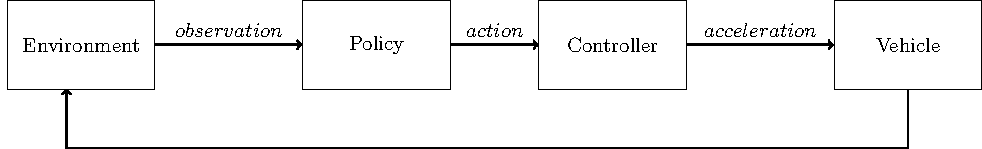
\includegraphics[width=0.9\columnwidth]{figures/figures-architecture.pdf}
	\caption{Representation of the architecture}
	\label{fig:Architecture}
\end{figure}\

Environment is defined as the world around the ego vehicle, including all vehicles of interest and the shape/type of the intersection. The environment can vary in different ways, e.g. number of vehicles and intersection or the distance to intersections. The environment is defined by the simulation explained in section \ref{sec:simulation}. We assume that the ego vehicle receives observations from this environment at each sampling instant, as shown in Fig. \ref{fig:Architecture}. A policy then takes these observations and chooses a high level action that is defined in more detail in section \ref{sec:observations}. These actions are sent to a controller that calculates the appropriate acceleration request given to the ego vehicle, which will influence the environment and impact how other cars behave. 

\subsection{Actions as Short Term Goals}
\label{sec:actions}
Motivated by the insight that the ego vehicle has to drive before or after other vehicles when passing the intersection, decisions on the velocity profile is modeled by simply keeping a distance to other vehicles until they pass. This is done by defining the actions as Short Term Goals (STG), eg. keep set speed or yield for crossing car. 
This allows the properties of comfort on actuation and safety to be tuned separately, making the decision a classification problem. 
The actions are then as followed:
\begin{itemize}
	\item \textit{Keep set speed}: Aims to keep a specified maximum speed $v_{\max}$, using a simple P-controller
	
	\begin{equation}
	a^e_p = K (v_{max} - v^e)
	\label{eq:p_control}
	\end{equation}
	
	where $a^e_p$ is the acceleration request and $v^e$ is the velocity of ego vehicle towards the center of the intersection, while $K$ is a proportional constant. 
	
	\item \textit{Keep distance to vehicle $N$}: Will control the acceleration in a way that keeps a minimum distance to a chosen vehicle $N$, a {\em Target Vehicle}, and can be done using a sliding mode controller, where the acceleration request is:
	
    \begin{equation}
    	a^e_{sm} = \frac{1}{c_2} (- c_1 x_2 + \mu sign(\sigma(x_1, x_2))) 
    	\label{eq:sliding_mode}
    \end{equation}
    
    $$
    \text{where}
    \begin{cases}
    x_1 = p^t - p^e \\
    x_2 = v^t - v^e
    \end{cases}
    $$

    where $p^e$ and $p^t$ is the position of ego and target vehicle respectively, shown in Fig. \ref{fig:Observations}, and $v^t$ is the velocity of target vehicle. $c_1$ together with $c_2$ are calibration parameters that can be set to achieve wanted performance with a surface plane $\sigma$
    
    \begin{equation}
    	\sigma = c_1 x_1 + c_2 x_2
    \end{equation}
    
    The final acceleration request $a^e$ is achieved by a min arbitration between eq. \ref{eq:p_control} and \ref{eq:sliding_mode} 
    
    \begin{equation}
		a^e = \min(a^e_{sm}, a^e_p )
		\label{eq:control}
    \end{equation}

    For more detailed information about sliding mode see \cite{MemonAnalysisManoeuvers}. % This controller could also be replaced with a Model Predictive Controller. 
    To distinguish between different cars to follow, each other vehicle will have its own action. 
    
    \item \textit{Stop in front of intersection}: Stops the car at the next intersection. Using the same controller as eq. \ref{eq:control} while setting $v^t = 0$ and $p^t$ to start of intersection, the controller can bring ego vehicle to a comfortable stop before the intersection. 
	
\end{itemize}
\subsection{Observations that make up the state}
\label{sec:observations}
\begin{figure}[!h]
	\centering
	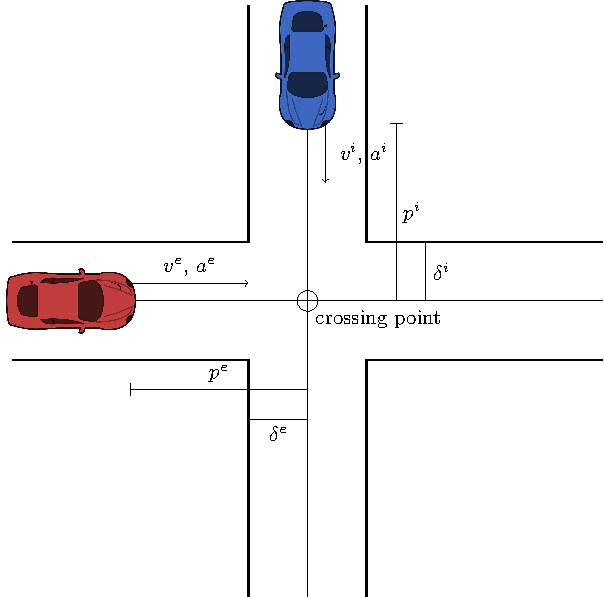
\includegraphics[width=0.6\columnwidth]{figures/figures-observations.pdf}
	\caption{Observations that makes the state}
	\label{fig:Observations}
\end{figure}

%Modellen bestämmer states (system), actions (system), reward function ("implicit" regulator) och gamma ("implicit" regulator)
%
%State förklaras från sina features. förklara features. med en figure

%Assuming the state is not directly known, some observations of the environment are used to estimate the state. 
A human driver is, generally, good at assessing a scenario and it is hard to pin-point what information is used in their assessment. Therefore some assumptions are made on which features that are interesting to observe. The observation $o_t$ at time $t$ is defined as:

\begin{equation}
o_t = [\  p^e_t \quad v^e_t \quad a^e_t \quad \delta^e \quad p^i_t \quad v^i_t \quad a^i_t \quad \delta^i \quad a^{e, A}_{t+1} \  ]^T
\end{equation}

With notations as follows: consider Fig. \ref{fig:Observations}, position of ego $p^e_t$ and other vehicle $p^i_t$ are defined as distance to common reference point, called {\em crossing point}, where $i$ is an index of the other vehicle. 
The start of intersection for ego $\delta^e$ and other vehicle $\delta^i$ also uses the crossing point as reference. These are relevant in case a driver would choose to yield for other vehicles, then they would most likely stop before the start of intersection. The velocity $v^e$ and acceleration $a^e$ of ego vehicle and velocity  $v^i$ and acceleration $a^i$ of the other vehicles are observed to include the dynamics of different actors. The last feature in the observation, $a^{e, A}_{t+1}$, is the ego vehicle's predicted acceleration for each possible action $A$, which can be used to account for comfort in the decision.

%The observations that represent the MDP state are the velocity of ego and target vehicle $v_{e}$, distance to crossing point of ego $d_{e}$ and target vehicle $d_{t}$ , the acceleration of the ego vehicle $a_{e}$. Distance to start of intersection for ego $d_{intersection}^e$ and target vehicle $d_{intersection}^t$.

\subsection{Partially Observable Markov Decision Processes}
The decision making process in the intersection is modeled as a POMDP. A POMDP works like a Markov Decision Process (MDP) \cite{BellmanMDP} in most aspects, but the full state is not observable. 

At each time instant, an action, $a_t\in \mathcal{A}$, is taken, which will influence to which new state vector, $s_{t+1}$, the system evolves and changes the environment. Each action $a_t$ from a state $s_t$ has a value called the reward $r_t$, which is given by a reward function $\mathcal{R}_t $.

One of the unobservable states could be the intentions of other drivers approaching the intersection. The state can only be perceived partially through observations $o_t\in \Omega$ with the probability distribution of receiving observation $o_t$ given an underlying hidden state $s_{t}: o_t \leftarrow \mathcal{O}(s_{t})$, where $\mathcal{O}(s_t)$ is the probability distribution. 

\section{Finding the optimal policy}
\label{sec:policy} 
Assuming the states are not known, we want a model-free method of finding a policy, and for this we use reinforcement learning. The goal is to have an agent learn how to maximize the future reward by taking different actions in a simulated environment. Details on the simulation environment used is described in Section \ref{sec:simulation}. The strategy of which action to take given a state is called a policy $\pi$ and can be modeled in two ways: 

\begin{itemize}
	\item As stochastic policy $\pi(a|s) = \mathcal{P}[\mathcal{A}=a|\mathcal{S}=s]$
	\item As deterministic policy $a = \pi(s)$
\end{itemize}
%TODO: add epislon greedy
The standard assumption is made that the future reward is discounted by a factor $\gamma$ per time step, making the discounted future reward $\mathcal{R}_t = \sum_{t}^{\tau} \gamma^{t-1} r_t$, where $\tau$ is the time step where the simulation ends, e.g. when the agent crosses an intersection safely. 

Similar to \cite{MnihPlayingLearning}, the optimal action-value function $Q^*(s_t, a_t)$ is defined as the maximum expected reward achievable by following a policy $\pi$ given the state $s_t$ and taking an action $a_t$:

\begin{equation}
Q^*(s_t,a_t)= \max_{\pi} \mathbb{E}[\mathcal{R}_t | s_t, a_t, \pi]
\end{equation}

%Knowing  $Q^*(s_t, a) \quad \forall a \! \in \! \mathbb{A}$,  $Q^*(s_t, a)$ can be defined recursively using the bellman equation. The optimal policy $\pi^*$ will then be one that takes an action $a_{t}$ that gives the highest immediate and discounted expected future reward $r_t + \gamma Q^*(s_{t+1}, a_{t+1})$.

Using the Bellman equation, $Q^*(s_t, a_t)$ can be defined recursively. If we know $Q^*(s_t, a)$ for all actions $a$ that can be taken in state $s_t$, then the optimal policy will be one that takes the action $a_{t}$ that gives the highest immediate and discounted expected future reward $r_t + \gamma Q^*(s_{t+1}, a_{t+1})$. This gives us: 

\begin{equation}
Q^*(s_t,a_t)= \mathbb{E}[r_t + \gamma \max_{a_{t+1}} Q^*(s_{t+1}, a_{t+1})| s_t, a_t]
\label{eq:q-function}
\end{equation}

The optimal policy $\pi^*$ is then given by taking actions according to an optimal $Q^*(s_t,a_t)$ function: 
\begin{equation}
\pi^*(s_t) = \arg\max_{a_t} Q^*(s_t,a_t)
\label{eq:optimal_policy}
\end{equation}

\section{Method}
\label{sec:method}
From eq. \ref{eq:optimal_policy}, the optimal policy is defined by taking an action that has the highest expected Q-value. Because the Q-value is not known, a non linear function approximation, such as a neural network, is used to estimate the Q-function. The method is known as Deep Q-Learning \cite{MnihPlayingLearning} and in this section we will briefly describe Q-learning and methods used to improve the learning such as, Experience replay, dropout and Long-, Short- Term Memory (LSTM).

\subsection{Deep Q-learning}
\label{sec:dqn}
Deep Q-Learning uses a neural network to approximate the $Q$-function. This neural network is called Deep Q-Network (DQN). The $Q$-function approximated by the DQN is denoted as $Q(s_t,a_t|\theta^\pi)$, where $\theta^\pi$ are the neural network parameters for policy $\pi$. The state $s_t$ is the input to the DQN and the output is the $Q$-value for each action $\mathcal{A}$.

\subsection{Experience Replay}
A problem with Deep Q-Learning, looking at eq. \ref{eq:optimal_policy}, is that with a small change in the $Q$-function, can effect the policy drastically. The distribution of future training samples will be greatly influenced by the updated policy. If the network only trains on recent experiences, a biased distribution of samples is used. Such behavior can cause unwanted feedback loops which can lead to divergence of the trained network \cite{Tsitsiklis1997AnApproximation}.

Proposed by \cite{MnihPlayingLearning} in order to make DQN more robust, all observations $o$, together with taken actions $a$ and their rewards $r$, are stored in an experience memory $E$ and the agent can sample experiences $E'$ from the experience memory. The sampled experiences are fed to the gradient descent algorithm as a mini-batch. Thus, the agent learns on an average of the experiences in $E$ and is likely to train on the same experiences multiple times, which can speed up the network's convergence and reduce oscillations \cite{Lin1992Self-ImprovingTeaching}.

\subsection{Dropout}
Overfitted neural networks have bad generalization performance \cite{Hinton2012ImprovingDetectors} and to help reduce overfitting a technique called dropout was used. The idea with dropout is to temporarily remove random hidden neurons with their connections from the network, before each training iteration. This is done by, independently, for each neuron, setting its value to 0 with a probability $p$. For more details, see \cite{Srivastava2014Dropout:Overfitting}. 

%The back propagation algorithm is updated accordingly. A network used in a training iteration will contain a subset of the neurons from the full neural network. There are an exponential number of these subsets, and back propagation with dropout can be seen as an algorithm training all those sub-networks. The final network will become an average of all sub-networks. During validation, all neurons are present but their weights are multiplied by $p$. This makes the expected output of the network during validation the same as during training. Dropout breaks the co-adaptation between hidden neurons, since they cannot assume that all other neurons are present. Therefore, each neuron generally becomes more useful.

\subsection{Long short term memory}
The effect of changes over time is explored in this paper and is done by adding a recurrent layer to the DQN making it a Deep Recurrent Q-Network (DRQN). A regular Recurrent Neural Network struggle to remember longer sequences due to vanishing gradients, and in \cite{Hochreiter1997LONGMEMORY} LSTM is used to solve this problem. 
%, which means that the gradients decrease exponentially for each unrolled time step. 
An LSTM is a recurrent network constructed for tasks with long-term dependencies. Instead of storing all information from previous time sample, LSTM stores information in a memory cell and modify this memory by using insert and forget gates. These gates decides if a memory cell should be kept or cleared, and during training, the network learns how to control these gates. As a result of this, both newly seen observations and observations seen a long time ago can be stored and used by the network. A sequence length of 4 is used when training the LSTM, where the first 3 observations are only used to build the internal memory state of the LSTM cells, as described in \cite{LamplePlayingLearning}.


%A hidden layer in an LSTM consists of four fully connected internal layers that together creates an output $\bm{h}_t$ and an internal cell state $\bm{C}_t$, which are both remembered between observations. The cell state is modified by inserting data to it or by removing remembered data. Two of the internal layers are the forget gate layer $\bm{f}_f$ and the insert gate layer $\bm{f}_i$. They both return a vector containing values between 0 and 1, where each value describes how important that element is in $\bm{C}_t$. For the forget layer, a 1 will keep the remembered data and a 0 will forget it. The layers are using a sigmoid activation function $\sigma(x)$ and will later be used for an element-wise multiplication (denoted by $\odot$) with the cell state \cite{Hochreiter1997LONGMEMORY}:
%
%\begin{gather*}
%\bm{f}_f = \sigma(\bm{W}_f \bm{z}_t + \bm{b}_f) \\
%\bm{f}_i = \sigma(\bm{W}_i \bm{z}_t + \bm{b}_i)
%\end{gather*}
%
%A candidate for the new cell state, $\bm{\tilde{C}}_t$, is computed from $\bm{z}_t = (\bm{\xi}_t \, || \, \bm{h}_{t-1})$, where $||$ denotes a concatenation. The cell state $\bm{C}_t$ is updated by passing the old cell state $\bm{C}_{t-1}$ through the forget gate and the candidate cell state $\bm{\tilde{C}}$ through the insert gate \cite{Hochreiter1997LONGMEMORY}:
%
%\begin{gather*}
%\bm{\tilde{C}}_t = \tanh(\bm{W}_C \bm{z}_t + \bm{b}_C) \\
%\bm{C}_t = \bm{f}_f \odot \bm{C}_{t-1} + \bm{f}_i \odot \bm{\tilde{C}}_t
%\end{gather*}
%
%The output of the cell, $\bm{h}_t$, contains selected values from the cell state. Another sigmoid layer, $\bm{f}_o$, is used to filter what parts of $\bm{C}_t$ to include in the output \cite{Hochreiter1997LONGMEMORY}:
%
%\begin{gather*}
%\bm{f}_o = \sigma(\bm{W}_o \bm{z}_t + \bm{b}_o) \\
%\bm{h}_t = \bm{f}_o \odot \tanh(\bm{C}_t)
%\end{gather*}
%
%A memory for $\bm{C}_t$ and $\bm{h}_t$ stores these values for the next observation. A network can contain multiple LSTM cell layers. In that case, each cell has its own memory and computes $\bm{h}_t$ based on its own $\bm{C}_{t-1}$ and $\bm{h}_{t-1}$. The parameters for an LSTM cell are $\theta = \{\bm{W}_f, \bm{W}_i, \bm{W}_C, \bm{W}_o, \bm{b}_f, \bm{b}_i, \bm{b}_C, \bm{b}_o\}$, which are trained using back propagation by unrolling each layer over time, similar to a normal RNN \cite{Hochreiter1997LONGMEMORY}.

\section{Implementation}
\label{sec:implementation}
In this section we go through the experiment implementation. A simulation environment was set up to model the interactions. From section \ref{sec:model}, both the number of observations and actions are dependent on the maximum number of cars. In this paper we consider up to 4 cars. The Deep Q Network can then also be fully defined with the help of observations from section \ref{sec:model} and finally we go though the reward function that defines our behavior. 

\subsection{Simulation environment}
\label{sec:simulation}
The simulation environment is set up as an intersection described in section \ref{sec:observations}. The number of other cars that are observable at the same time can vary from 1-4, while their intentions can vary between an aggressive {\em take way}, passive {\em give way} or a cautious driver. The take way driver does not slow down or yield for crossing traffic in an intersection, while the give way driver will always yield for other vehicles before continuing through the intersection. The cautious driver on the other hand, will slow down for crossing traffic but not come down to a full stop. With a maximum number of other cars set to 4 all possible actions the ego vehicle can take are:

\vspace{0.2cm}
\begin{itemize}
	\item $\alpha_1$: Keep set speed.
	\item $\alpha_2$: Stop in front of intersection.
	\item $\alpha_3$: Keep distance to vehicle 1.
	\item $\alpha_4$: Keep distance to vehicle 2.
	\item $\alpha_5$: Keep distance to vehicle 3.
	\item $\alpha_6$: Keep distance to vehicle 4.
\end{itemize}
\vspace{0.2cm}

At the start of an episode, the ego vehicle's position and velocity, the number of other vehicles and their intentions are randomly generated. The episode only end when the ego vehicle fulfills one out of  three conditions: 1. Crossing the intersection and reaching the other side, 2. Colliding with another vehicle. or 3. Running out of time $\tau_m$. Each car follows the control law from eq. \ref{eq:control}, trying to keep a set speed while keeping a set distance to the vehicle in front of its own lane. 

All cars including the ego vehicle in these scenarios have a maximum acceleration set to $5 m/s^2$ and was set after comfort and normal driving conditions. 

\subsection{Reward function tuning}
When using a DQN, the reward function is optimally distributed around $[-1, 1]$. If the defined reward values are too large, the $Q_\pi$-values can become large and cause the gradients to grow \cite{VanHasseltLearningMagnitude}. 
The reward function is defined as follows:
\begin{align*}
r_t = \hat{r}_t + &\begin{cases}
1 - \frac{\tau}{\tau_m} & \text{on success, }\\
-2                 & \text{on collision}\\
-0.1                & \text{on timeout, i.e. } \tau \ge \tau_m\\
-\left(\frac{j^{e}_t}{j_{\max}}\right)^2\frac{\Delta \tau}{\tau_m}         & \text{on non-terminating updates}
\end{cases} \\
\text{where } \hat{r}_t = &\begin{cases}
-1  & \text{if chosen $a_t$ is not valid}\\
0   & \text{otherwise}
\end{cases}
\end{align*}

\noindent The actions $\alpha_3, \dots, \alpha_6$ described should only be selected when a vehicle is visible and a valid target to follow. To learn when these action are valid, the agent gets punished on invalid choices using $\hat r_t$. Accelerations returned by the controller for different STG can vary, which increases jerk and can make the ride uncomfortable. Therefore the reward function also punishes the agent when acceleration jerk $j^{e}_t$ is large, where $\tau$ is the elapsed time sense the episode started and $\tau_m$ is the maximum time has before a timeout. 

\subsection{Neural Network Setup}
%features, shared weights, LSTM in the end. figure on network setup. Figure \ref{fig:network}
\begin{figure}[!t]
	\centering
	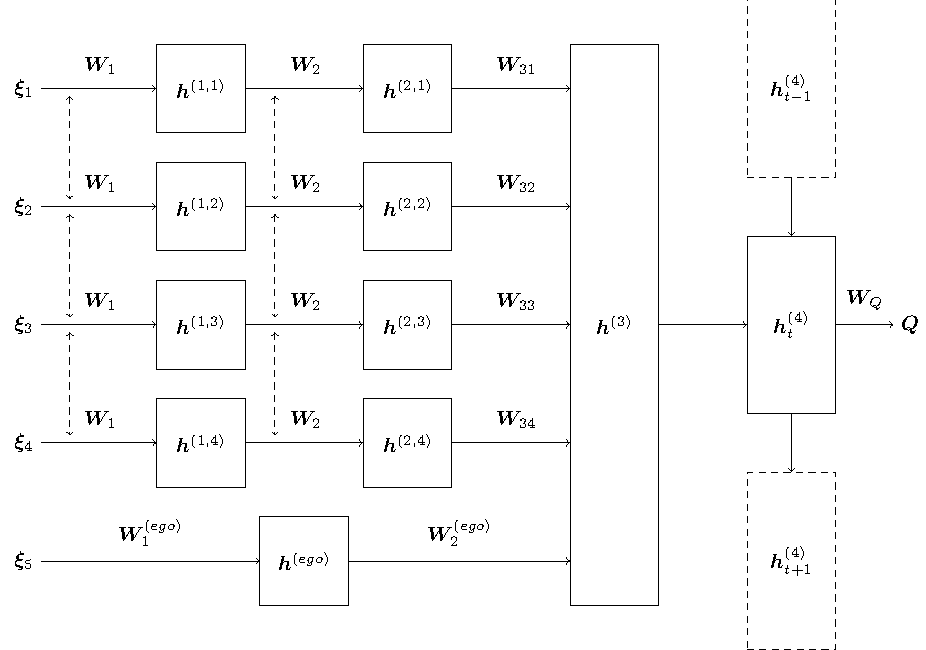
\includegraphics[width=0.95\columnwidth]{figures/figures-network.pdf}
	\caption{Deep Recurrent Q Network layout with shared weights and a LSTM}
	\label{fig:network}
\end{figure}

The DRQN structure is defined in Fig. \ref{fig:network}. Where $\bm{h}$ are the hidden layers of the network with weights $\bm{W}$. Because the observations $o_t$ from section \ref{fig:Observations}, are used as input to the DRQN, the number of features must be fixed. With up to four other cars the input vectors $\bm{\xi}$ are as follows:
\vspace{0.3cm}
\begin{itemize}
	\item $ \xi_1 = [\  p^e_t \quad v^e_t \quad a^e_t \quad \delta^e \quad p^1_t \quad v^1_t \quad a^1_t \quad \delta^1 \  ]^T$
	\item $ \xi_2 = [\  p^e_t \quad v^e_t \quad a^e_t \quad \delta^e \quad p^2_t \quad v^2_t \quad a^2_t \quad \delta^2 \  ]^T$
	\item $ \xi_3 = [\  p^e_t \quad v^e_t \quad a^e_t \quad \delta^e \quad p^3_t \quad v^3_t \quad a^3_t \quad \delta^3 \  ]^T$
	\item $ \xi_4 = [\  p^e_t \quad v^e_t \quad a^e_t \quad \delta^e \quad p^4_t \quad v^4_t \quad a^4_t \quad \delta^4 \  ]^T$
	\item $ \xi_5 = [\  a^{e, 1}_{t+1} \quad a^{e, 2}_{t+1} \quad a^{e, 3}_{t+1} \quad a^{e, 4}_{t+1} \quad a^{e, 5}_{t+1} \quad a^{e, 6}_{t+1} \  ]^T$
\end{itemize}
\vspace{0.3cm}
In case a vehicle is not visible, the input vector $\bm{\xi}$ are set to -1. All vehicle features are scaled to be a value between or close to $[-1,1]$ by using a car's sight range $p_{\max}$, maximum speed $v_{\max}$ and maximum acceleration $a_{\max}$.

%The vehicle features are listed below:
%\begin{itemize}
%	\item $\xi_1$: \textbf{vehicles 1's position relative to ego vehicle}, using the other vehicle's position along the ego lane: $$\frac{p^e_t  + p^1_t }{p_{\max}}$$
%	\item $\xi_2$: \textbf{Vehicle 1’s speed}, $\frac{v^1_t }{v_{\max}}$
%	\item $\xi_3$: \textbf{Vehicle 1’s acceleration}, $\frac{a^1_t }{a_{\max}}$
%	\item $\xi_4$: \textbf{Vehicle 1's distance to start of intersection}. $$\frac{p^1_t - \delta^1 }{p_{\max}}$$
%	\item $\xi_5$: \textbf{Ego vehicle’s speed}, $\frac{v^e_t}{v_{\max}}$
%	\item $\xi_6$: \textbf{Ego vehicle’s acceleration}, $\frac{a^e_t}{a_{\max}}$
%	\item $\xi_7$: \textbf{Ego vehicle’s distance to start of intersection}: $$\frac{p^e_t - \delta^e }{p_{\max}}$$
%	\item $\xi_8$: \textbf{Ego car’s distance to overlap with target lane}. 
%	$$\frac{\phi^{(L_e)}_\circ - p^{(e)}_t}{p_{\max}}$$
%\end{itemize}

%To make the learning process faster and to improve performance, the network structure is modified to share some network weights. 
The output $\bm{Q}$ should be independent of which order other vehicles was observed in the input $\xi_i$. In other words, whether a vehicle was fed into $\xi_1$ or into $\xi_4$, the network should optimally result in the same decision, only based on the features' values. 
The network is therefore structured such that input features of one car, for instance $\xi_1$, are used as input to a sub-network with two layers$\bm{h}^{(1, i)}$ and $\bm{h}^{(2, i)}$. Each other vehicle has a copy of this sub-network, resulting in them sharing weights ($\bm{W}_1$ and $\bm{W}_2$), as shown in Fig. \ref{fig:network}. The first hidden layers are then given by:

\begin{equation}
\bm{h}^{(1, i)} = \tanh\left(\bm{W}_1 \bm\xi_i + \bm{b}_1\right)
\end{equation}
\begin{equation}
\bm{h}^{(2, i)} = \tanh\left(\bm{W}_2 \bm{h}^{(1, i)} + \bm{b}_2\right)
\end{equation}
\begin{equation}
\bm h^{(ego)}   = \tanh\left(\bm{W}^{(ego)}_{1}  \bm\xi_5 + \bm{b}^{(ego)}\right)
\end{equation}

The output of each sub-network, $\bm{h}^{(2, i)}$ and $\bm h^{(ego)}$,  is fed as input into a third hidden layer $\bm{h}^{(3)}$.
The different sub-networks' $\bm{h}^{(2, i)}$ outputs are multiplied with different weights $\bm{W}_{31},\dots,\bm{W}_{34}$ in order to distinguish different cars for different follow car actions. The ego features are also fed into layer 3 with its own weights $\bm{W}^{(ego)}_2$. The neurons in layer $\bm{h}^{(3)}$ combine the inputs by adding them together:

\begin{equation}
\label{eq:shared_weights}
\bm{h}^{(3)} = \tanh\left(\bm{W}^{(ego)}_{2} \, \bm h^{(ego)} + \sum_{i=1}^4 \bm{W}_{3i} \, \bm{h}^{(2, i)} + \bm{b}_3\right)
\end{equation}

The final layer $\bm{h}^{(4)}$ uses the LSTM, described in section \ref{sec:method}. This layer handles the storage and usage of previous observations, making it the recurrent layer of the network. 

\begin{equation}
\bm{h}^{(4)}_t = \text{LSTM}\left( \bm{h}^{(3)} | \bm{h}^{(4)}_{t-1} \right)
\end{equation}

The output of the neural network is then the approximated $\bm{Q}$-value:

\begin{equation}
\bm{Q} = \bm{W}_Q \bm{h}^{(4)}+ \bm{b}_4
\end{equation}

\section{Results}
\label{sec:results}
Three metrics were selected for measurement of a training session: success rate, average episodic reward and collision to timeout ratio. With these metrics, the distribution between the three terminating states can be analyzed. Success rate is defined as the success to fail ratio averaged over the last 100 episodes, where both collisions and timeouts are considered as failures. 
Average episodic reward is the summed reward over a whole episode, then averaged over 100 episodes. 
The collision to fail ratio displays the ratio between the number of collisions and unsuccessful episodes for the last 100 episodes. From the success rate and collision to fail ratio, a final collision rate is computed, which is the amount of episodes resulting in a collision, averaged over 100 episodes. 
%In each graph, there is a faded colored line that show actual sampled values, and a thick line that acts as a trend line. 
The graphs presented are only using evaluation episodes, with a deterministic policy. Every $300$ episode, the trained network is evaluated over $300$ evaluation episodes.

The improvement of using Dropout and Experience replay, from Section \ref{sec:method}, are clearly shown in Fig. \ref{fig:results_experience} and \ref{fig:results_dropout}. Studying the red curve in Fig. \ref{fig:results_experience}, with all methods included, the best policy had a success rate of $99\%$, average episodic reward $0.8$ and collision to timeout ratio at $40\%$. 

\subsection{Effect of using Experience replay}
\begin{figure}[!ht]
	\centering
	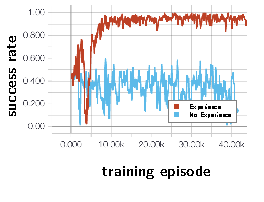
\includegraphics[width=0.7\columnwidth]{figures/figures-experience.pdf}
	\vspace{-0.5cm}
	\caption{Success rate trend comparing using experience replay (red) and not using experience replay (blue)}
	\label{fig:results_experience}
\end{figure}
Without either method the success rate does not converge to a value higher than $60\%$. When experience replay was not used, the highest success rate was $53\%$, average episodic reward $-0.1$ and collision to timeout ratio at $90\%$. Compared to not using dropout, not using experience replay has a higher lower variation on the success rate. 

\subsection{Effect of using Dropout}
\begin{figure}[!ht]
	\centering
	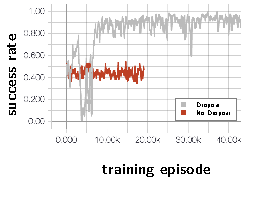
\includegraphics[width=0.7\columnwidth]{figures/figures-dropout.pdf}
	\vspace{-0.5cm}
	\caption{Success rate trend comparing using dropout (grey) and not using dropout (red)}
	\label{fig:results_dropout}
\end{figure}
In the case of not using Dropout, the best policy had a success rate of $58\%$, average episodic reward $-0.7$ and a collision to timeout ratio at $90 \%$. 


\subsection{Comparing DQN and DRQN}
\begin{figure}[!ht]
	\centering
	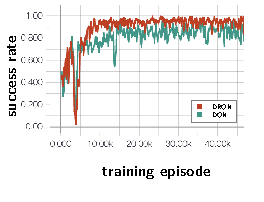
\includegraphics[width=0.7\columnwidth]{figures/figures-recurrent.pdf}
	\vspace{-0.5cm}
	\caption{Graphs presenting the performance of a DRQN (red) compared to a DQN with a single observation (green), running on scenarios with cars that have different behaviors. When compared a DRQN succeeds in 3 out of 4 attempts, where a DQN fails.}
	\label{fig:results_recurremt}
\end{figure}
In Fig. \ref{fig:results_recurremt}, we can see the effect off having a recurrent layer by comparing a DQN, without a LSTM layer, and  with a DRQN, with LSTM.
The faded colored line show actual sampled values and the thick line acts as a trend line which for DRQN converges towards a success rate of around 97.2\% and a 0.85\% collision rate, compared to a success rate of 87.5\% and a collision rate of 1.75\% for DQN. 


\subsection{Effect of sharing weights in the network}
\begin{figure}[!ht]
	\centering
	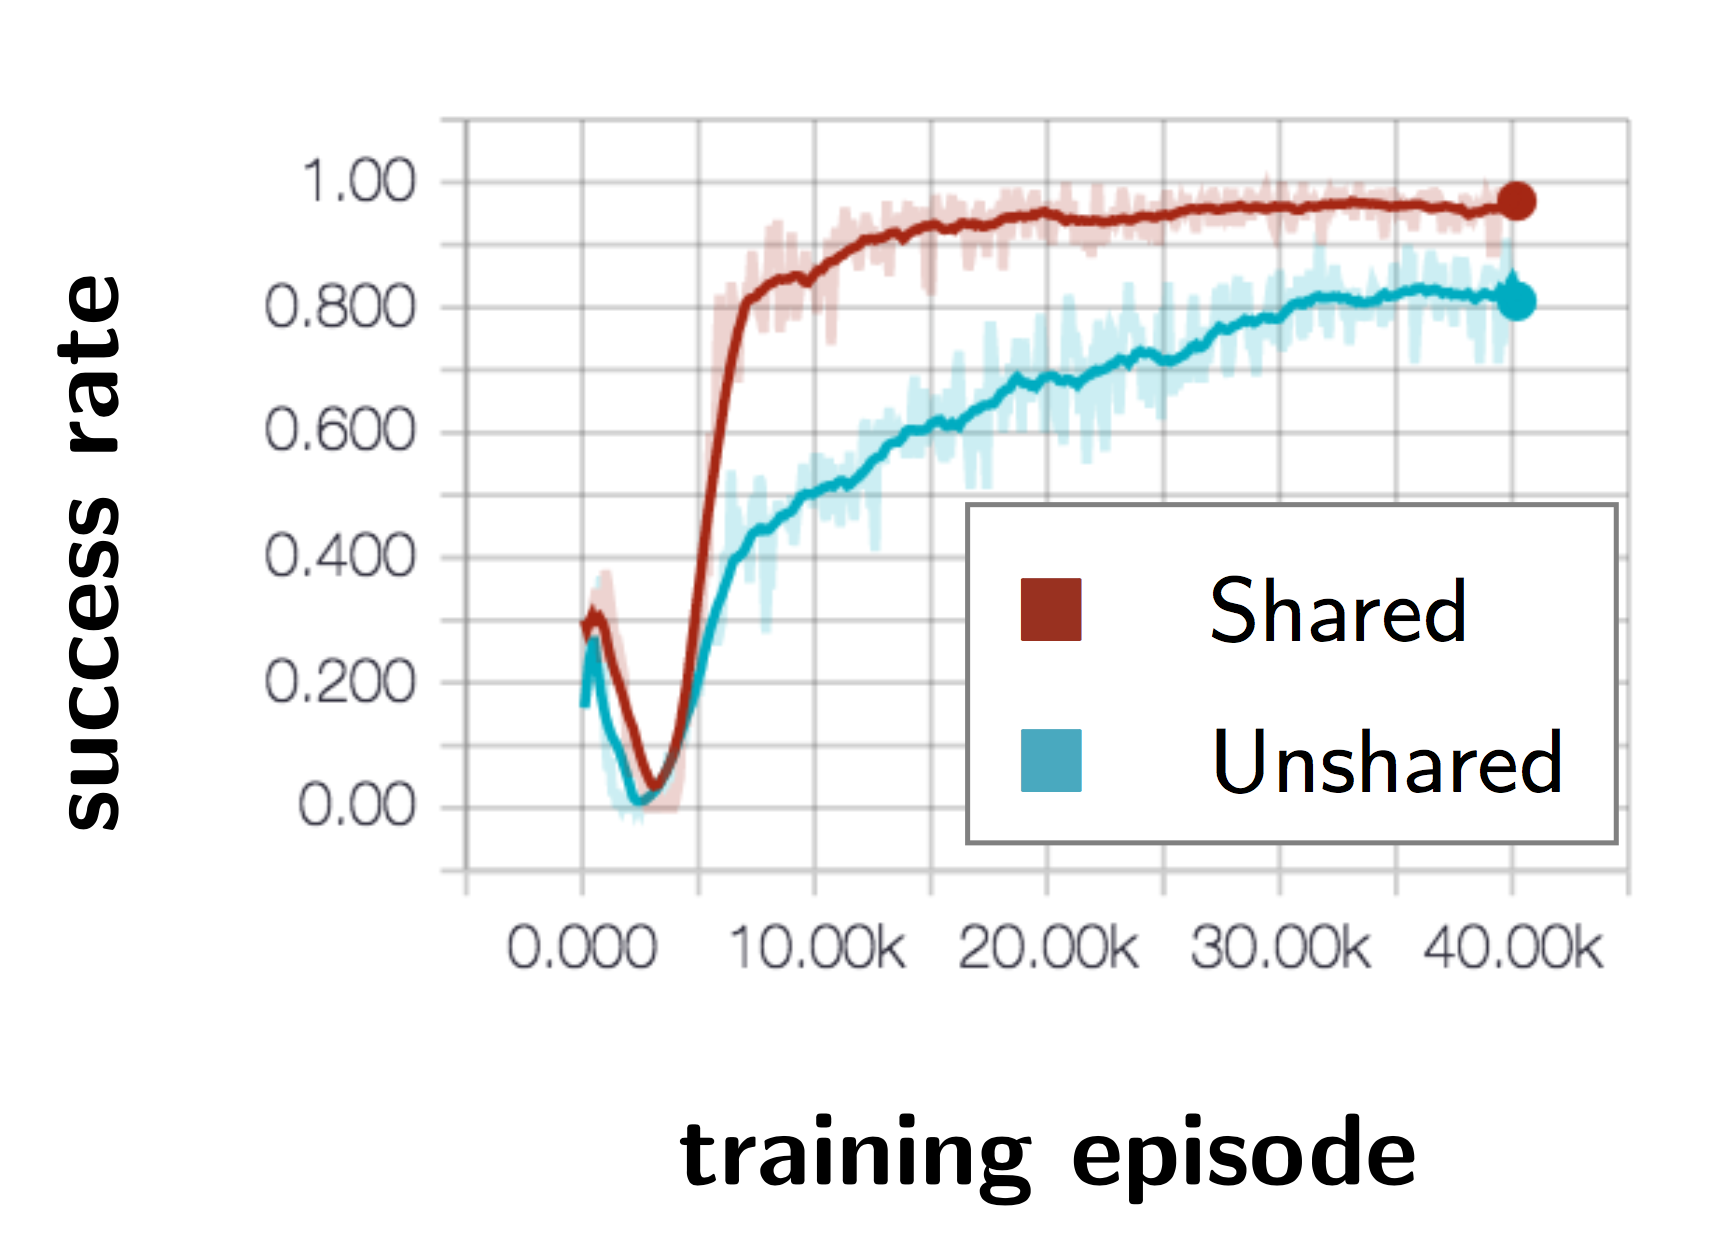
\includegraphics[width=0.8\columnwidth]{figures/results_shared.png}
	\caption{The figure shows that the success rate for a network with shared weights (brown line) converge faster than the fully connected network structure which do not share weights (turquoise line).}
	\label{fig:results_shared}
\end{figure}
When introducing multiple cars in the scenario, the success rate converged considerably slower, as shown in Fig. \ref{fig:results_shared}. Using the network structure that share weights between cars, significantly improved how fast the network converged compared to a fully connected DRQN. 

\section{Conclusion}
\label{sec:conclusion}
In this paper, Deep Q-Learning was presented in the domain of autonomous vehicle control. The goal of the ego agent is to drive through an intersection, by adjusting longitudinal acceleration using short-term goals. Short-term goals also allowed a smoother and more human-like behavior by controlling the acceleration and comfort with a separate controller. Instead of finding a policy with a continuous control output the problem became a classification problem. 

The results also show that trained policies can generalize over different types of driver behaviors. The same policy is able to respond to other vehicles' actions and handle traffic scenarios with a varied number of cars, without knowing traffic rules or the type of intersection it drives in. Multiple observations are needed in order to recognize cars' behaviors, and can be utilized by for instance a DRQN. 

There was a significant performance improvement in using a DRQN instead of a DQN with a single observation. In other words, the environment for these scenarios is better modeled as a POMDP instead of an MDP and the agent needs multiple observations in order to draw enough conclusions about other cars' behaviors.
Convergence of the neural network was shown to be improved by sharing weights between the first layers to which the target car features are fed, compared to a fully connected neural network structure.
The results are still limited to the tested traffic scenarios and driver behaviors, and expanding the domain beyond a simulator is a natural next step. The selected features are also limited to intersections. 

The results show a success rate of around 99\% for recognizing behaviors.  However, the ego vehicle still collides. The ego vehicle is limited to drive comfortably, meaning that in some cases, the ego agent is not allowed to break hard enough. In a complete system, a collision avoidance procedure, which does not have comfort constraints, would need to take over the control to ensure a safe ride.
A collision in this paper is defined by two areas overlapping, and in a real world implementation this does not have to mean an actual collision. Instead this could be interpreted as an intervention from a more safety critical system. This way, in the low chances a good action could not be found, the safety of the vehicles can still be guarantied. 

In section \ref{sec:actions}, a sliding mode controller was chosen, but this can be replaced by any controller. One other option could be a Model Predictive Controller, where safer actuation can be achieved by using constraints. Also, the actions in this paper used the same controller tuning for all actions, this does not have to be the case. An action can have the same STG but only differ by the controller's tuning parameters. This way, the agent gains more flexibility while the comfort can maintain intact, possibly increasing the success rate. 
